\section{Components}

To start, we split the project into a number of smaller modular components, that, when put together, make up a product that solves the requirements. The purpose of this is to gain an overview over the pieces of functionality required for the product, and the dependencies between these. Each component will be regarded as a wholly modular piece of the product, and will be tested separately from the rest. 

%Each component deals with only its own concerns

See figure \ref{fig:components} for the component diagram showing a separation of concerns into product components and their dependencies. On each component we've written the main functions that the component allows, abstracting away all low-level details. The arrows signify dependencies, e.g. that the manoeuvre-component requires the functions of the driving-component in order to work. 

\begin{figure}[ht]
    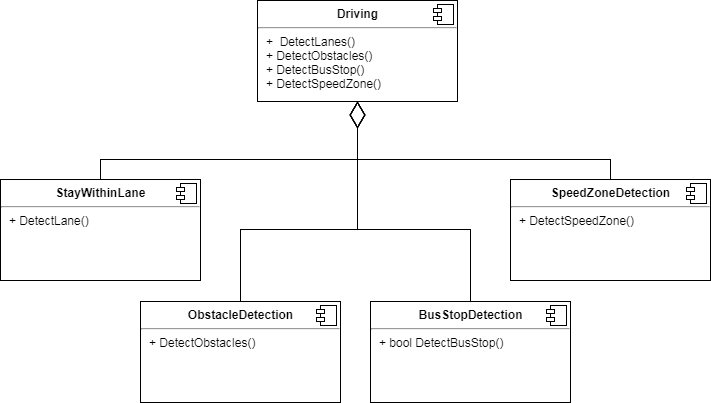
\includegraphics[width=\textwidth]{Images/Design/componentDiagram.png}
    \caption{Major components of functionality in the product; each component deals only with its own concerns}
    \label{fig:components}
\end{figure}
%Jeg er ikke overbevist om at ovenstående diagram er vildt vigtigt når vi nu alligevel har det nedenstående, dog giver det fint mening indtil videre

Note that the components refer not only to software, but also the physical design of the car. For instance, after we implement the driving component in software, we require a functioning LEGO-bus to test the software on. Only after this is done can we conclude whether the component works properly. Reason being that although the software logic might work as intended, incorrect sensor measurements, track/lane inconsistencies and similar need to be taken into account during programming, because otherwise the product might not work as expected.
